\chapter{Formalization of sequential decision making}
In this chapter we will dive into Markov Decison Process (MDP). First we’ll remind ourselves what it means for a process to be Markovian. Next we’ll add numerical rewards to that process and ask about total accumulated reward; that gives us a Markov reward process (MRP). Finally we allow an agent to choose actions that influence the transitions and the rewards; that gives us a Markov decision process (MDP). Formulating a learning problem as an MDP is the first step in applying reinforcement learning: once you have the MDP, you can ask “what policy maximizes expected return?” and start designing algorithms to learn that policy.

Many decision problems have delayed consequences: the action you take now affects not only the reward you receive immediately but also which states you’ll see later and therefore the future rewards you can obtain. The MDP framework forces you to model this sequential dependence explicitly and to think about trading off immediate against delayed reward.

Imagine an agent interacting with an environment at discrete time steps $t=0,1,2,\ldots$ At time $t$ the agent observes a state $S_t$ (a representation of the environment), chooses an action $A_t$, and then, one time step later, receives a numerical reward $R_{t+1}$ and lands in a new state $S_{t+1}$.

\section{Introduction to Markov Decison Process}
A state $S_t$ is called Markov if knowing $S_t$ makes everything from the full history irrelevant for predicting the future. Formally, a state sequence has the Markov property if
\begin{equation*}
    P(S_{t+1}|S_t) = P(S_{t+1}|S_1, S_2, \ldots, S_t).
\end{equation*}
In words: once you know the current state, the probability distribution of the next state does not depend on how the process arrived at the current state. The present is a sufficient statistic of the future. That is why we can “forget” the history and reason only about the current state and the transition probabilities from it.

If the state space $S$ is finite we can arrange all transition probabilities into a matrix. For two states $s$ (current) and $s'$ (next), the one-step transition probability is
\begin{equation*}
    P_{ss'} = P(S_{t+1}=s'|S_t=s).
\end{equation*}
The matrix $P$ with entries $P_{ss'}$ collects these probabilities for all pairs $s$, $s'$. Each row of $P$ is a probability distribution over next states given the current state, so each row sums to 1.

A Markov process (also called a Markov chain) can thus be compactly described as the pair $\langle S,P\rangle$: the set of states and the transition matrix.

\begin{Example}{Student Markov Chain}{}
Imagine a simple model of a student moving through states that describe the student’s academic day. 

Let's assume the student was taking \texttt{Class1} of the Autonomous Networking course. From this state, he can reach \texttt{Class2} with a probability of 0.5, and if bored by the lesson, he starts scrolling Facebook with a probability of 0.5. Here, the social network algorithm keeps him glued to the screen with a probability of 0.9, and he returns to the lesson only 10\% of the time. Obviously, the student's ultimate goal is to reach the \texttt{Pass} state to pass the exam. To do this, he will have to attend all three classes, avoiding to falling asleep during \texttt{Class2}, which is also the most difficult. In the meantime, he might consider taking a break from studying and going to the \texttt{Pub}. Here, he shouldn't overdrink, otherwise he'll forget the lessons learned in the classes and have to start over again.

\begin{minipage}{\textwidth}
    \centering
    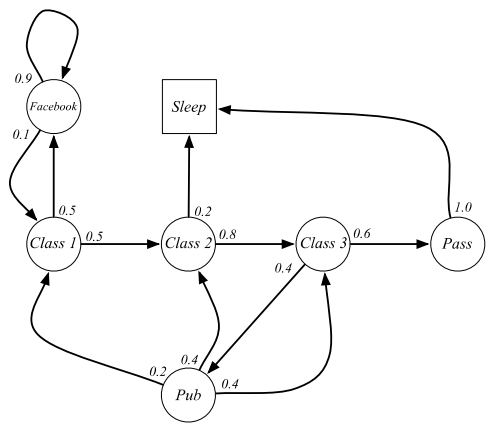
\includegraphics[width=0.7\linewidth]{images/student-markov-chain.png}
    %\captionsetup{hypcap=false}
    %\captionof{figure}{Query tree.}
    \label{fig:student-markov-chain}
\end{minipage}

Each state has probabilities of transitioning to certain successor states. From the transition matrix you can sample sequences such as
\begin{equation*}
    C_1 \to C_2 \to C_3 \to Pass \to Sleep,    
\end{equation*}
or
\begin{equation*}
    C_1 \to FB \to FB \to C_1 \to C_2 \to Sleep,    
\end{equation*}
or longer weird sequences like
\begin{align*}
    C_1 \to FB \to FB \to C_1 \to C_2 \to C_3 \to Pub \to C_1 \to FB \to FB \to FB \to C_1 \to C_2 \to C_3 \to\\ Pub \to C_2 \to Sleep.    
\end{align*}
Those sequences are just realizations of the Markov chain according to the probabilities in the transition matrix. When you simulate, the actual sequence depends on the random draws at each step but the distribution over sequences is completely defined by $P$.

A representation of the transition matrix $P$ of the student Markov chain example can be:
\[
P=\begin{bmatrix}
0   & 0.5 & 0   & 0   & 0   & 0.5 & 0   \\
0   & 0   & 0.8 & 0   & 0   & 0   & 0.2 \\
0   & 0   & 0   & 0.6 & 0.4 & 0   & 0   \\
0   & 0   & 0   & 0   & 0   & 0   & 1.0 \\
0.2 & 0.4 & 0.4 & 0   & 0   & 0   & 0   \\
0.1 & 0   & 0   & 0   & 0   & 0.9 & 0   \\
0   & 0   & 0   & 0   & 0   & 0   & 1.0
\end{bmatrix}
\]
with row-labels: \(C_{1},C_{2},C_{3},Pass,Pub,FB,Sleep\) and same order for column-labels.
\end{Example}

\section{Markov Reward Process}
A Markov reward process is simply a Markov chain with a numerical reward assigned to states (or transitions) as illustrated in Figure \ref{fig:markov-reward-process}. We write an MRP as the tuple $\langle S,P,R,\gamma\rangle$. Here $S$ and $P$ are as before, $R$ is a reward function and $\gamma$ is a discount factor.

\begin{figure}[ht]
    \centering
    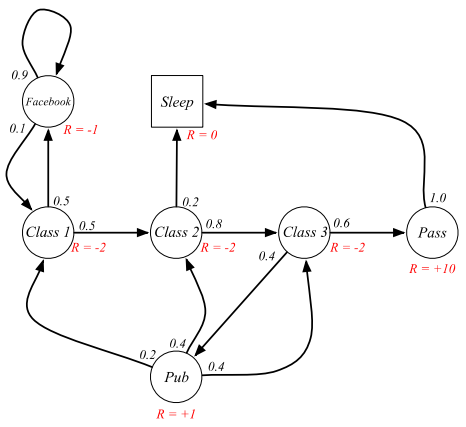
\includegraphics[width=0.7\linewidth]{images/student-markov-reward-process.png}
    \caption{Markov Reward Process in the student example.}
    \label{fig:markov-reward-process}
\end{figure}

The reward function $R$ is commonly given as the expected immediate reward when in state $s$:
\begin{equation*}
    R_s = E[R_{t+1}|S_t=s].
\end{equation*}
Being in state $s$ at time $t$ leads to receiving reward $R_{t+1}$ on the transition to $t+1$.

The discount factor $\gamma$ is a number in the interval $[0,1]$ which defines how future rewards are valued relative to immediate rewards. We’ll explain its role in a moment.

When we evaluate what happens from time $t$ onward we care about the sequence of future rewards. The return $G_t$ is defined as the total discounted reward from time $t$:
\begin{equation*}
    G_t=R_{t+1}+\gamma R_{t+2}+\gamma^2R_{t+3}+\ldots = \sum_{k=0}^\infty\gamma^kR_{t+k+1}.    
\end{equation*}
Discounting multiplies a reward received $k$ steps in the future by $\gamma^k$. If $\gamma = 0$ the agent is completely myopic and only considers the immediate reward. If $\gamma$ is near 1 the agent is far-sighted and cares about long-term consequences.

Why do we include a discount factor? Several reasons. Discounting is mathematically convenient because it ensures the infinite sum is finite in many cyclic or continuing processes. Practically it expresses a preference for rewards sooner rather than later, models uncertainty about long-term outcomes, and sometimes corresponds to economic notions of time preference. In episodic tasks (where sequences terminate) it is sometimes appropriate to set $\gamma = 1$, but for continuing tasks the discount is usually strictly less than 1.

The state value function $v(s)$ gives the expected return when starting in state $s$. Formally,
\begin{equation*}
    v(s) = E[G_t|S_t=s].
\end{equation*}
Because $G_t$ is a sum of discounted future rewards, $v(s)$ captures the long-run goodness of being in state $s$, taking into account future transitions and rewards.

If $\gamma=0$ the value function ignores future rewards entirely and reduces to the immediate reward. Whatever reward you get immediately in state $s$ is the value $v(s)$. If $\gamma=0.9$ (a moderately high discount), the value $v(s)$ combines the immediate reward and substantial weight on rewards a few steps ahead. The value of states that are likely to lead to \texttt{Pass} or other high-reward states will increase, while states likely to lead to \texttt{FB} or \texttt{Sleep} will have lower value. If $\gamma=1$ (no discounting, appropriate only when episodes terminate or when the sum is known finite), the value becomes the expected undiscounted sum of future rewards. This makes long term prospects weigh exactly the same as near-term ones, so states that eventually lead to a lot of reward are very valuable even if the reward is delayed.

\begin{figure}[ht]
    \centering
    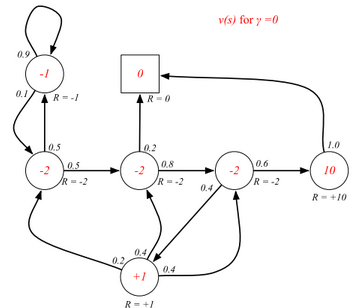
\includegraphics[width=0.45\linewidth]{images/state-value-func-student1.png}
    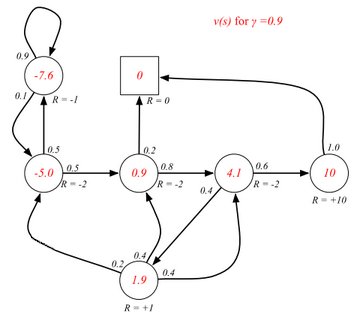
\includegraphics[width=0.45\linewidth]{images/state-value-func-student2.png}
    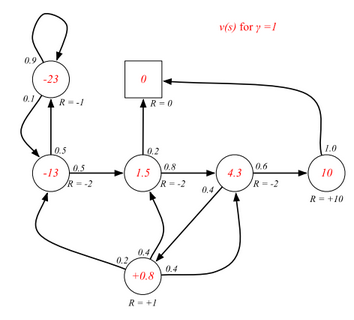
\includegraphics[width=0.45\linewidth]{images/state-value-func-student3.png}
    \caption{State-Value Function for Student MRP.}
    \label{fig:state-value-func-student.png}
\end{figure}

The value of a state and the value function can be split into two parts. If you are in state $s$ the total value function $v(s)$ equals the immediate reward you get on the next transition, $R_{t+1}$, plus the discounted value from the next state, $\gamma v(S_{t+1})$:
\begin{align*}
    v(s)&=E[G_t|S_t=s]\\
    &=E[R_{t+1}+\gamma R_{t+2} + \gamma^2 R_{t+3 + \ldots}|S_t=s]\\
    &=E[R_{t+1}+\gamma (R_{t+2} + \gamma R_{t+3 + \ldots}|S_t=s]\\
    &=E[R_{t+1}+\gamma G_{t+1}|S_t=s]\\
    &=E[R_{t+1}+\gamma v(S_{t+1})|S_t=s].
\end{align*}
future value is just an expected, discounted copy of the same quantity evaluated one time-step later.

Because the environment is stochastic, there may be many possible successor states and many possible rewards when you start from $s$. The Bellman equation averages over all these possibilities, weighting each by its probability. In words it says: the value of the starting state must equal the expected immediate reward plus the discounted expected value of where you end up next.
The value of a state is tied to the values of its successors.

Start from the definition $v(s)=E[G_t|S_t=s]$ and substitute $G_t=R_{t+1}+\gamma G_{t+1}$. Then 
\begin{equation*}
    v(s)=E[R_{t+1}+\gamma G_{t+1}|S_t=s].    
\end{equation*}
The expectation of the sum is the sum of expectations. The immediate reward expectation is $R_s = E[R_{t+1}|S_t=s]$. The second term is 
$\gamma$ times the expected return from the next state: $\gamma\sum_{s'\in S}P_{ss'}v(s')$, because the next state is $s'$ with probability $P_{ss'}$ and from there the expected future return is $v(s')$. Put together:
\begin{equation*}
    v(s)=R_s+\gamma\sum_{s'\in S}P_{ss'}v(s').    
\end{equation*}
That is the canonical Bellman equation for an MRP.

\begin{figure}[ht]
    \centering
    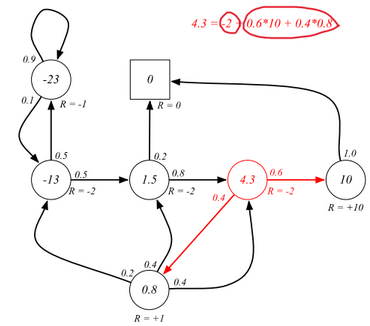
\includegraphics[width=0.5\linewidth]{images/bellman-student.png}
    \caption{Bellman equation applied to the student example with $\gamma=1$.}
    \label{fig:bellman-student}
\end{figure}

It’s often cleaner to write the Bellman equation in vector/matrix notation. Let $v$ be the column vector whose entries are $v(s)$ for each state 
$s$. Let $R$ be the column vector with entries $R_s$. Let $P$ be the transition matrix with entries $P_{ss'}$. Then the Bellman equation for the MRP becomes 
\begin{equation*}
    v=R+\gamma Pv.
\end{equation*}
This single vector equation contains all state equations at once. You can rearrange it into the familiar linear-algebra form $(I-\gamma P)v=R$.
If $I-\gamma P$ is invertible, the closed-form solution is:
\begin{align*}
    v&=R+\gamma Pv\\
    (I-\gamma P)v&=R\\
    v&=(I-\gamma P)^{-1}R
\end{align*}
The Bellman equation is a linear system in the unknowns $v(s)$. For a state space of size $n$, solving the linear system directly by matrix inversion or Gaussian elimination has computational complexity roughly $O(n^3)$. That is fine for small MRPs but quickly becomes infeasible when 
$n$ is large.
Because of this, a variety of iterative methods are used for larger problems. Dynamic programming gives iterative policy-evaluation procedures that converge to the exact $v$ when you have a complete model. Model-free methods such as Monte Carlo evaluation approximate values by sampling complete returns, and temporal-difference (TD) methods like TD(0) bootstrap the current estimate against sampled immediate rewards plus a discounted next-state value. All of these are ways to solve or approximate the Bellman equations without inverting a huge matrix.

\section{Markov Decison Process}
A Markov decision process is exactly a Markov reward process with actions: the environment is fully observable, all states are Markov, and the agent chooses actions that influence the next-state distribution and the immediate reward.

Formally, an MDP is the tuple $\langle S,A,P,R,\gamma\rangle$. The set $S$ is the finite set of states. $A$ is the set of actions; the transition matrix is $P_{ss'}^a = P(S_{t+1}=s'|S_t=s,A_t=a)$, and $R_s^a = E[R_{t+1}|S_t=s,A_t=a]$.

There is effectively one transition matrix per action. If you think of $P$ as a block of matrices, each action $a$ supplies a matrix $P^a$ that tells you how the environment responds to that action across all states.

In the student MDP the states are the same as before, but now the agent chooses actions in some states: for instance the agent can choose to study or check Facebook. Each action might lead to different immediate rewards and different transition probabilities. The goal is to choose actions along the way so that the accumulated discounted reward is maximized.

\subsection{Policy}
A policy fully defines the agent’s behavior. A policy $\pi$ maps states to distributions over actions; formally
\begin{equation*}
    \pi(a|s) = P(A_t=a|S_t=s).
\end{equation*}
Policies are typically assumed stationary: the distribution depends on the current state but not on time. Stationarity makes the math simpler and often suffices for many tasks, though time-dependent policies can appear in certain contexts.

When a policy $\pi$ is fixed, an MDP becomes an MRP: the stochastic dynamics together with the policy create effective transition probabilities and expected rewards (you marginalize over the actions chosen by $\pi$).

\subsection{Value function}
For a given policy $\pi$ the state-value function $v_\pi(s)$ is the expected return starting in state $s$ and following $\pi$ afterwards:
\begin{equation*}
    v_\pi(s)=E_\pi[G_t|S_t=s].
\end{equation*}
The action-value function $q_\pi(s,a)$ measures the expected return starting from state $s$, taking action $a$ once at that state, and then following $\pi$ thereafter:
\begin{equation*}
    q_\pi(s,a)=E_\pi[G_t|S_t=s,A_t=a].    
\end{equation*}
These two functions are linked by the simple identity
\begin{equation*}
    v_\pi(s)=\sum_{a\in A}\pi(a|s)q_\pi(s,a),
\end{equation*}
which simply says the value of a state under $\pi$ is the average, under $\pi$, of the action-values for that state.

You can write Bellman-style recursive equations for both $v_\pi$ and $q_\pi$. The state-value Bellman expectation equation decomposes $v_\pi(s)$ into the expected immediate reward plus the discounted expected value of the successor state, where the expectation averages both over the policy’s action distribution and the environment’s transition distribution. Formally:
\begin{equation*}
    v_\pi(s)=\sum_{a \in A} \pi(a|s)\left(R_s^a+\gamma\sum_{s'\in S}P_{ss'}^av_\pi(s')\right).
\end{equation*}
You can see this as first choosing an action with probability $\pi(a|s)$; given that action, you get immediate expected reward $R_s^a$ and then move to $s'$ with probability $P_{ss'}^a$, from which you get value $v_\pi(s')$.

The action-value Bellman expectation equation is similar, but it conditions on having taken action $a$ in the current state:
\begin{equation*}
    q_\pi(s,a)=R_s^a+\gamma\sum_{s'\in S}P_{ss'}a\sum_{a'\in A}\pi(a'|s')q_\pi(s',a').    
\end{equation*}
Here the inner sum $\sum_{a'\in A}\pi(a'|s')q_\pi(s',a')$ is simply $v_\pi(s')$, hence the action-value equation can be written as
\begin{equation*}
    q_\pi(s,a)=R_s^a+\gamma\sum_{s'\in S}P_{ss'}^av_\pi(s').
\end{equation*}

\section{Optimal policy}
A policy is simply a way for an agent to behave: given the current state, the policy tells the agent what action to take (deterministically or stochastically). Up to now, we’ve often treated a policy as something that was given, and the task was to evaluate it — to compute the value function that tells us how good that policy is.

Reinforcement learning, however, has a more ambitious goal. We don’t only want to evaluate a single policy; we want to discover the best policy possible. That is, we want a policy that, across time, gathers as much cumulative reward as possible. The rest of this chapter is about formalizing what “best” means, how to express it, and how to compute it.

To compare two policies we look at their value functions. A policy $\pi$ is considered better than or equal to another policy $\pi'$ if for every state $s$ the expected return starting from $s$ under $\pi$ is at least as large as under $\pi'$. In symbols we write $\pi \geq \pi'$ when $V_\pi(s) \geq V_{\pi'}(s)$ for all $s$.
Because of this partial ordering, we can ask whether there exists a policy that is better than or equal to every other policy. The answer is yes. For any Markov Decision Process (MDP) there exists at least one policy $\pi_*$ such that $\pi_* \geq \pi$ for every policy $\pi$. That policy $\pi_*$ is called an optimal policy.
All optimal policies share the same optimal value functions (state-value and action-value), so finding those value functions is the key to finding optimal behavior.

Two central objects are the optimal state-value function $v_*$ and the optimal action-value function $q_*$.
The optimal state-value function $v_*(s)$ is defined as the maximum state-value achievable from state s by any policy:
\begin{equation*}
    v_*(s) = \max\pi V_\pi(s).    
\end{equation*}
This expresses the best possible expected return you can guarantee when starting from state $s$. The optimal action-value function $q_*(s,a)$ is defined similarly but conditions on taking a specific action $a$ in state $s$ first:
\begin{equation*}
q_*(s,a) = \max_\pi q_\pi(s,a).    
\end{equation*}
In words, $q_*(s,a)$ tells you the best expected return you can achieve if you start in state $s$, take action $a$ now, and then follow the best possible policy afterwards.

If you have $q_*(s,a)$, finding an optimal policy is immediate: in each state choose an action that maximizes $q_*$:
\begin{equation*}
    \pi_*(a|s) = 
    \begin{cases}
        1 & if a = argmax_{a \in A} q_*(s,a)\\
        0 & otherwise
    \end{cases}
\end{equation*}
Because the $argmax$ may not be unique, there can be multiple optimal policies, but they all have the same values $v_*$ and $q_*$. Importantly, there always exists at least one deterministic optimal policy for any finite MDP — so you can pick a single best action in every state and be optimal.

\subsection{Bellman Optimality Equation}
The optimal value functions satisfy recursive identities called the Bellman optimality equations. They are the same flavor as the Bellman equations for a fixed policy, but here we take the maximum over actions because we allow the agent to choose the best action at each step.

The optimal value functions satisfy recursive identities called the Bellman optimality equations. They are the same flavor as the Bellman equations for a fixed policy, but here we take the maximum over actions because we allow the agent to choose the best action at each step.

The Bellman optimality equation for the optimal state-value $v_*$ is:
\begin{equation*}
    v_*(s) = \max_a E[R_{t+1}+\gamma v_*(S_{t+1})|S_t=s,A_t=a],    
\end{equation*}
or, written explicitly in terms of transition probabilities,
\begin{equation*}
    v_*(s) = max_a \sum_{s', r}p(s',r|s,a)[r+\gamma v_*(s')].
\end{equation*}
Read this as: the value of the best action in state $s$ equals the expected immediate reward from that action plus the discounted value of the next state, where we then assume we continue optimally.

The Bellman optimality equation for the optimal action-value $q_*$ is similar but starts from a state–action pair:
\begin{equation*}
    q_*(s,a) = E[R_{t+1}+\gamma max_{a'} q_*(S_{t+1},a')|S_t=s,A_t=a],    
\end{equation*}
or explicitly
\begin{equation*}
    q_*(s,a) = \sum_{s',r} p(s',r|s,a) [r+\gamma max_{a'} q_*(s',a')].
\end{equation*}
This says: the value of taking action $a$ in state $s$ equals the expected immediate reward plus the discounted value of the best action available in the next state.

\subsection{Solving the Bellman Optimality Equation}
The Bellman optimality equation is the precise mathematical statement of “act optimally at every step.” It tells us, for each state or state–action pair, what the optimal value must equal. But there’s a catch. The equation is nonlinear because it contains a max over actions. That nonlinearity means there is no general closed-form solution you can write down for $v_*$ or $q_*$ in an arbitrary MDP. Instead we solve it iteratively.

There are several well-known iterative families of methods. If you know the model (the transition probabilities and rewards), dynamic programming gives elegant and reliable algorithms; policy iteration alternates between evaluating a policy and improving it; if you don’t know the model and must learn from experience, you use sample-based methods such as Q-learning or Sarsa (and more generally TD-based methods). Each of these algorithms is a way of repeatedly applying the Bellman operator (or an approximation of it) until the value estimate stabilizes.

\subsubsection{Temporal-Difference (TD) learning}
Temporal-Difference learning is a family of methods that learn value functions directly from experience. The key idea is: instead of waiting until an entire episode finishes to compute a return, update value estimates using the difference between successive predictions — that is, the prediction error you see after one time step.

If you are estimating a state value function $V_\pi$ for a fixed policy $\pi$, TD methods address the prediction problem: given observed transitions generated using $\pi$, how should you update your estimate of $V_\pi$? At each time step, you have the previous estimate for the current state, you observe the immediate reward and the next state, and you compute a one-step target from that observation. The difference between that one-step target and your old estimate is called the TD error; it tells you how much to adjust the old estimate.

The simplest TD method is TD(0), also called one-step TD. It’s a special case of the more general TD($\lambda$) family, and it forms the building block for TD control algorithms like Q-learning.

\begin{Example}{Driving-home story}{}
    Imagine every day you try to predict how long the drive home will take. In the morning you say “30 minutes.” Halfway there you’re stuck in traffic and realize 30 minutes was optimistic. Do you have to wait until you arrive to adjust your initial prediction? TD says: no. As soon as you get information (say, a traffic jam report or a much slower speed on the road), you update your prediction for the starting point using that intermediate information. TD(0) is exactly that — you update estimates step by step as new observations arrive, using the most recent successor as a sample of the next state.
\end{Example}

For state-value prediction TD(0) uses this update:
\begin{equation*}
    V(S_t)\rightarrow V(S_t)+\alpha[R_{t+1}+\gamma V(S_t+1) - V(S_t)].
\end{equation*}
Here $\alpha$ is the learning rate, $R_{t+1}$ is the reward observed after leaving $S_t$, and $\gamma$ is the discount factor. The bracketed term is the TD error: the one-step target $R_{t+1}+\gamma V(S_{t+1})$ minus the old estimate $V(S_t)$. Notice TD(0) uses a single sampled successor rather than the full expected distribution over successors; that’s what makes it sample-based.

\begin{lstlisting}[mathescape]
Input: the policy $\pi$ to be evaluated
Algorithm parameters: step size $\alpha\in [0, 1]$
Initialize $V(s)$, for all $s\in S^+$, arbitrarily except that $V$ (terminal) = 0

Loop for each episode:
    Initialize $S$
    Loop for each step of episode:
        $A \rightarrow$ action given $\pi$ for $S$
        Take action $A$, observe $R, S'$
        $V(S) \rightarrow V(S) + \alpha[R + \gamma V(S') - V(S)]$
        $S \rightarrow S'$
    until $S$ is terminal
\end{lstlisting}
\captionof{lstlisting}{Tabular TD(0) for estimanting $v_\pi$}

\subsubsection{Q-learning}
Q-learning is a TD method extended to the control problem: it directly learns estimates of the optimal action-value function $q_*(s,a)$ from experience, without needing a model.

Q-learning is an off-policy TD control algorithm. “Off-policy” means the policy used to generate behavior (the behavior policy) can be different from the policy being evaluated and improved (the target policy). Concretely, while the agent might explore randomly or follow an exploratory policy to collect data, Q-learning always updates its table toward the greedy target (the max over next-state actions). This makes Q-learning a very flexible algorithm: you can explore arbitrarily and still learn the optimal $q_*$.

The TD error for Q-learning uses the standard one-step target but with a max over next actions. For a transition $(S_t,A_t,R_{t+1},S_{t+1})$ the TD error is
\begin{equation*}
    \delta_t = R_{t+1} + \gamma \max_a Q(S_{t+1},a) - Q(S_t,A_t).
\end{equation*}
Think of this term piecewise. The first part, $R_{t+1}$, is the immediate reward received after taking action $A_t$ in state $S_t$. The second part, $\gamma\max_aQ(S_{t+1},a)$, is the discounted estimate of the best possible future value from the next state. Subtracting the current estimate $Q(S_t,A_t)$ yields the error — how far the current $Q$ is from the one-step backed-up target.

The Bellman equation for optimal $Q$ implies that, in expectation and at convergence, $\delta_t$ will be zero for every state–action pair.

Q-learning applies the TD error with a step size $\alpha$:
\begin{equation*}
    Q(S_t,A_t)\rightarrow Q(S_t,A_t)+\alpha \delta_t,    
\end{equation*}
which expanded is
\begin{equation*}
    Q(S_t,A_t)\rightarrow Q(S_t,A_t)+\alpha[R_{t+1}+\gamma\max_aQ(S_{t+1},a) - Q(S_t,A_t)].
\end{equation*}
The update mixes the old value with a new sample-based target. The learning rate $\alpha$ controls how much weight you give the new sample. If 
$\alpha$ is 1 you jump fully to the sample target (unstable); if $\alpha$ is very small you learn slowly. 

You can read the Q-learning update as an application of a Bellman backup: the new desired value for the state–action pair $(s,a)$ is the immediate reward plus the discounted value of the best action in the successor state. The algorithm uses the sampled successor to approximate that expected backup. Over many visits and with sufficient exploration, these sample backups approximate the expectation and $Q$ converges to the fixed point that satisfies the Bellman optimality equation for $q_*$.

\begin{lstlisting}[mathescape]
Algorithm pararmeters: step size $\alpha\in [0, 1]$, small $\epsilon > 0$
Initialize $Q(s, a)$, for all $s\in S^+$, $a\in A(s)$, arbitrarily except that $Q$ (terminal, $\cdot$) = 0

Loop for each episode:
    Initialize $S$
    Loop for each step of episode:
        Choose $A$ from $S$ using policy derived from $Q$ (e.g. $\epsilon$-greedy)
        Take action $A$, observe $R, S'$
        $Q(S, A) \rightarrow Q(S, A) + \alpha[R + \gamma\max_a Q(S', a) - Q(S, A)]$
        $S \rightarrow S'$
    until $S$ is terminal
\end{lstlisting}
\captionof{lstlisting}{Q-learning (off-policy TD control) for estimating $\pi\approx\pi_*$.}